%%%%%%%%%%%%%%%%%%%%%%%%%%%%%%%%%% PREAMBLE %%%%%%%%%%%%%%%%%%%%%%%%%%%%%%%%%%%%

\documentclass{uvamscse}	% UvA thesis class

% numeric citations, name/title/year sorting
%\usepackage[backend=biber, style=alphabetic, citestyle=alphabetic, sorting=nty]{biblatex}

% program listings environment, see uvamscse.cls
\usepackage{listings}

\lstdefinelanguage{sdf}{%
  numbers=none,
  morekeywords={module,imports,exports,sorts,context,lexical,free,syntax,==,=,+,-,left,cons,prefer,avoid,bracket},
  columns=flexible,
  morestring=[b]",
  basicstyle=\footnotesize\mdseries,
  literate={->}{{\,\,$\to$\,\,}}1
}

\lstdefinelanguage{dcg}{%
  numbers=none,
  morekeywords={},
  morestring=[b]",
  basicstyle=\footnotesize\mdseries,
  columns=flexible,
}

\lstdefinelanguage{prolog},
  literate={:-}{{\,$\Leftarrow$\,\,}}1 {-->}{{$\to$\,}}1
}

\lstdefinestyle{mono}{
  basicstyle=\footnotesize\ttfamily
}

\lstset{%
  frame=none,
  xleftmargin=2pt,
  stepnumber=1,
  numbers=left,
  numbersep=7pt,
  numberstyle=\ttfamily\scriptsize\color[gray]{0.3},
  belowcaptionskip=\bigskipamount,
  captionpos=b,
%  escapeinside={*'}{'*},
  % language=fl,
  tabsize=2,
  emphstyle={\bf},
  stringstyle=\itshape,
  showspaces=false,
  keywordstyle=\bfseries\rmfamily,
  columns=flexible,
  basicstyle=\small\mdseries,
  showstringspaces=false,
}

\newcommand{\cmd}[1]{\texttt{$\backslash$#1}}

\title{Detecting Online Conversations Going Viral}
\coverpic[250pt]{figures/Buzzcapture_thunder.png}
\subtitle{Time-series aware evaluation of change detection algorithms}
\date{Spring 2017}

\author{Matt Chapman}
\authemail{matthew.chapman@student.uva.nl}
\host{Buzzcapture International, \url{http://www.buzzcapture.com}}
\supervisor{Evangelos Kanoulas, Universiteit van Amsterdam}

\abstract{
	\todo[inline]{Write abstract}
}

\begin{document}
\nocite{*}
\maketitle

%%%%%%%%%%%%%%%%%%%%%%%%%%%%%%%%%%%%%%%%%%%%%%%%%%%%%%%%%%%%%%%%%%%%%%%%%%%%%%%%

\chapter{Problem Statement \& Motivation}

\section{Problem Statement}

Within the domain of change detection algorithms there are a number of available methods for evaluating the efficiency and accuracy of a given algorithm, depending on how the problem is framed. The different problem framings available are, for example:\unsure{are these definitions correct?}

\begin{description}
	\item[Classification] Wherein the algorithm result fits into one of two (or more) classes, for example correct or incorrect.
	\item[Clustering] Wherein the algorithm results are formed into clusters and evaluated using clustering metrics.
	\item[Partitioning] Wherein the data set is segmented according to change point location, and then evaluated in a similar way to clustering.
	\item[Retrieval] Wherein the results of the algorithm are scored as a \emph{retrieval problem}, where detection relevance is taken into account, perhaps along with some form of temporal or redundancy penalty.
\end{description}

With this research it is intended to investigate this dichotomy between approaches and examine how they perform with relation to evaluating the performance of change detection algorithms, specifically when applied to time-series data from social media.

While change detection itself has been around since the 1930's (and \emph{online} change detection since the 1950's) it is still a field that attracts new thoughts and approaches - one example of which being Ginsberg et. al.'s work on Influenza outbreak detection \cite{Ginsberg2009}.

Various attempts have been made to evaluate the myriad approaches to change detection (\cite{Buntain2014} for example) but each of these attempts tend to frame the problem somewhat differently.

This research intends to address the following research questions:

\todo[inline]{These will change later in the project}

\begin{description}
	\item[RQ1] Are there deficiencies in existing methods for evaluating change detection algorithms?
	\item[RQ2] Do certain measures perform better as an evaluation method when applied against changes detected in a data stream with certain properties?
	\item[RQ3] Is there room for adjustment in existing measures, such that they can be made more effective for the evaluation of change detection algorithms?
\end{description}

\improvement[inline]{this needs expansion, I think}

\section{Motivation}

Change detection first came about as a quality control measure in manufacturing, and methods within this domain are generally referred to as \emph{control charts}. Since the inception of approaches such as CUSUM that provide the possibility for on-line evaluation of continuous data streams, change detection has grown as a field. With applications such as epidemic detection, online reputation management and infrastructure error detection, change detection is hugely useful both as an academic problem and in production systems of myriad application.

This particular research is motivated specifically by the online reputation management sector. The business hosting this research project (Buzzcapture International [\url{http://www.buzzcapture.com}]) is a Dutch online reputation management company that provides services to other businesses throughout Europe. Chief among these is the BrandMonitor application, which, among other features, provides a rudimentary notification system for clients that is triggered once there is an increase in conversation volume of $\%n$. It is the intention of this research to provide a robust evaluation method for change detection algorithms such that an approach that is most effective for this particular use case can be selected and implemented.

The problem that this research sets out to address, is to examine how well certain evaluation measures correlate to real-world performance of the evaluated algorithms. For example, if the PELT algorithm is particularly "effective" and (correctly) supplies a set of changepoints for a given data set, yet these detections do not look right when examined ``by eye'', can the algorithm really be said to be effective? Are there situations where evaluation measures disagree with each-other and provide conflicting results?

\chapter{Research Method}

\section{Introduction}

Being that this research is analysing not just change detection algorithms themselves, but also the approaches to evaluation that exist

\section{Existing Approaches}

As briefly discussed in the introduction to this thesis, there are a number of pre-existing approaches for the evaluation of change detection methods. Here some examples are detailed:

\begin{description}
	\item[F1 Score]\unsure{cite this?} This measure is utilised for testing accuracy in problems of binary classification. It considers two	different measures, \emph{precision} and \emph{recall}. The F1 score can be described in general terms as follows:

	\begin{equation}
		F_1 = 2 \cdot \frac{1}{\frac{1}{recall} + \frac{1}{precision}} = 2 \cdot \frac{precision \cdot recall}{precision+recall}
		\label{equ:F1}
	\end{equation}

	$recall$ is computed as the number of correct positive results, divided by the number of positive results that should have been detected. $precision$ is computed as the number of correct positive results divided by the number of all possible positive results.

	As the F1 score is a binary classification measure, it can only be used to test the precision of an algorithm in a single domain, that is, was the change detected or not.

	\item[Rand Index] This measure is for computing the similarity between two clusters of data points. It is generally considered an accuracy score for clustering mechanisms. The Rand Index is defined as:

	\begin{equation}
		R = \frac{a+b}{a+b+c+d}
	\end{equation}

	Given a set of elements $S$ which is partitioned according to two different methods $X$ and $Y$, $a$ refers to the number of pairs of elements that exist in the same subset in both $X$ and $Y$, $b$ refers to the number of pairs of elements that exist in different subsets in both $X$ and $Y$, $c$ refers to the number of pairs of elements which exist in the same subset of $X$ and a different subset in $Y$, and $d$ refers to the number of pairs of elements that exist in different subsets in $X$ and the same subsets in $Y$. Intuitively, it can be stated that $a+b$ represents the number of agreements between $X$ and $Y$, and $c+d$ represents the number of \emph{disagreements} between $X$ and $Y$.\todo{this reads horribly, and is paraphrased from wikipedia. Need to find the proper source for this and rewrite}
	
	\item[Adjusted Rand Index]Similar to the Rand Index, but where the Rand Index is suited for comparing a segmentation method against a known-good \emph{oracle} method, the adjusted index is more suited to comparing two differing approaches.\todo{CITE! I read this somewhere, should find it again} It is defined as:
	
	\begin{equation}
	    R_{adjusted} = \frac{R - R_{expected}}{R_{max} - R_{expected}}
	\end{equation}

\end{description}

\section{Evaluation Pipeline}

\subsection{Introduction}

The method of evaluating the approaches will be developed using \textsf{R}. \textsf{R} is a combined language and environment created for the purpose of statistical computing \cite{RCoreTeam2017}. Thanks to the availability of the \texttt{changepoint} package in \textsf{R}\cite{Killick2014}, it is possible for me to experiment with different change detection approaches without needing to implement them from scratch, myself.

\textsf{R} also allows for the generation of test data using method calls such as \texttt{rnorm()}, which has considerably sped up my workflow compared to carrying out the same operations in Python. The \textsf{R} package \texttt{ggplot2} \cite{Wickham2009} also provides a number of powerful tools for data visualisation directly in \textsf{R}.

\subsection{Changepoint}

\texttt{changepoint} is a powerful R package that provides a number of different change detection algorithms, along with various approaches to penalty values. \texttt{changepoint} offers change detection in mean, variance and combinations of the two, using the AMOC, PELT, Binary Segmentation and Segment Neighbourhood algorithms\todo{cite these}.

\texttt{Changepoint} was developed by Rebecca Killick and Idris A. Eckley\todo{cite} and is provided free of charge under the GNU general public license.

\section{Data Preparation}

There are two data sets that will be used in this research. The first is a collection of 30.9M Dutch language tweets collected between 01/01/2017 and 28/02/2017. The data will be filtered for certain terms in the tweet 'body' to generate collections of tweets that would be considered 'relevant' to a particular business or individual. In this way, I will be able to simulate BrandMonitor queries myself, without the need of the software itself.

%\begin{figure}[hbt]
%	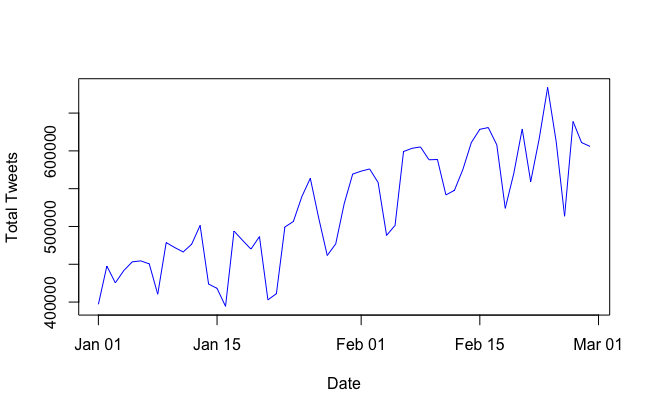
\includegraphics[scale=0.5]{figures/twitter-totals-full.png}
%	\centering
%	\caption{Twitter Data Set}
%	\label{fig:totals_graph}
%\end{figure}

\improvement[inline]{Make graph prettier}

The final result of the prepared data\todo{finish getting data together} shall be 5 different subsets of varying size and nature. For example, data sets with large changes in variance (noise), and extremely large/small changes in mean.

\subsection{The Nature of Twitter Data}

It is important, as part of this research, to understand the nature of the data being studied. The main reason for this is that several of the algorithms being evaluated require one to specify either a test statistic or the distribution of the data (as closely) as possible to give optimal results. For example, for detection of changes in mean using the \texttt{changepoint} package, one must specify whether the data follows a normal distribution, or whether to use the CUSUM (cumulative sum) test statistic that makes no assumptions about the distribution of the data.

%\begin{figure}[hbt]
%	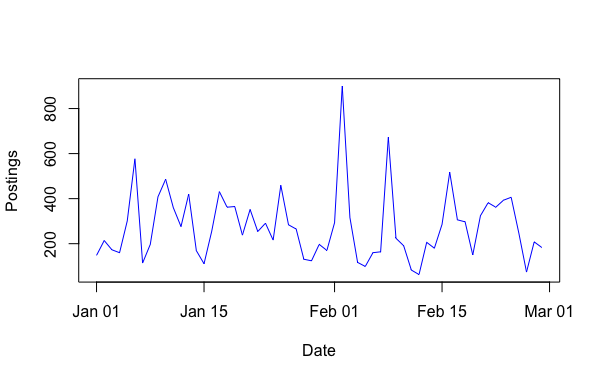
\includegraphics[scale=0.5]{figures/ing-totals-full.png}
%	\centering
%	\caption{"ING" postings by date}
%	\label{fig:ing_totals_graph}
%\end{figure}

Figure \ref{fig:ing_totals_graph} shows the distribution of twitter postings mentioning ``ING'' between 01/01/2017 and 28/02/2017. At first glance, this data has a number of interesting change points that we may wish to detect. Firstly, we shall examine what kind of distribution this data falls under. Carrying out the Shapiro-Wilk normality test gives us a \emph{p-value} of 0.0001037, well below the normally accepted 0.05. We can further see that this data set does not fit a normal distribution by generating a Q-Q plot of the data using R. \ref{fig:ing_QQ_plot} shows the completed QQ plot, which demonstrates the lack of normal distribution.

%\begin{figure}[hbt]
%	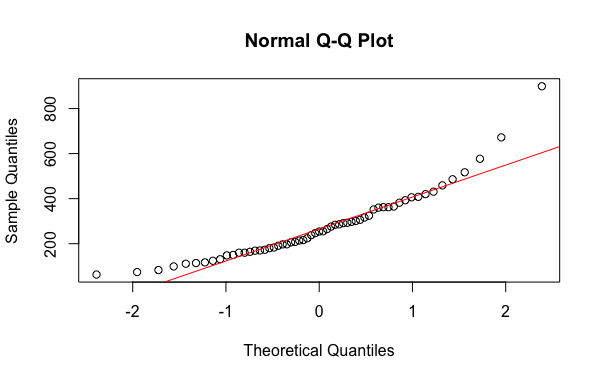
\includegraphics[scale=0.5]{figures/qqplot-ing.png}
%	\centering
%	\caption{Q-Q plot of ING postings}
%	\label{fig:ing_QQ_plot}
%\end{figure}

The second type of data that will be used is entirely simulated. This will be achieved using R's facilities for generating sets of random data that fits a normal distribution. In this way it will be possible to demonstrate how (if at all) change detection algorithms handle data with different distribution models differently.

\section{Algorithm Configuration}

Change detection is an \emph{unbounded} problem. Left without some system of constraint, the algorithm could theoretically run to infinity. Indeed, one of the algorithms utilised in this research, PELT\todo{citation needed}, when left unbounded, will detect every data point in the time-series as a change point. This result is \textit{technically} correct, but not useful for our purposes. For this reason, the algorithms implement a penalty system, allowing for an optimal number of changepoints to be detected.

\subsection{Penalty Scores}

Penalty scores operate as a mechanism for optimising an unbounded problem such as the one being addressed here. Haynes et al. define the problem as follows \cite{Haynes2014}: Given time series data points $y_1,\ldots,y_n$, the result of a given algorithm shall be a set of $m$ changepoints such that their locations $\tau_{1:m} = (\tau_1,\ldots,\tau_m)$, where $\tau_i$ is an integer between 1 and $n-1$ inclusive.

\begin{equation}
    Q_m(y_{1:n}) = \min_{\tau_{1:m}} \{ \sum^{m+1}_{i=1}[C(y_{(\tau_{i - 1} + 1):\tau_i})] \}
\end{equation}

There are a number of established approaches to calculating penalty values for unbounded problems, chiefly among which are Schwarz Information Criterion (SIC), Bayesian Information Criterion (BIC), Akaike Information Criterion (AIC) and Hannan-Quinn\todo{cite}. Of these approaches, it is necessary to experiment to find the scheme that produces the `correct' number of changepoints for a given dataset.

\section{Scoring Metrics}

\subsection{F1 Score}

The first calculated metric is \emph{F1 Score}, which is described by the equation \ref{equ:F1}. We calculate F1 score in the following manner:

For a given structure of time series data $S$ such that the points in the series are $(x_{t:0},\ldots,x_{t:n})$, we create two lists of points: $P$ and $T$. $P$ represents the set of changepoints predicted by the algorithm being evaluated, and $T$ represents the \emph{ground truth}, the changepoints annotated by a domain expert\todo{further explanation}. Both lists contain only $0$ and $1$, $0$ being a point where no changepoint is predicted, and $1$ being a point where a changepoint is predicted. In this manner we frame the changepoint detection problem as a binary classification problem.

From these data structures $P$ and $T$ we can easily compute precision as $\frac{\sum (P \wedge T) }{\sum P}$ and recall as $\frac{\sum (P \wedge T)}{\sum T}$. These values can then be inserted into equation \ref{equ:F1} to obtain the F1 score.

\subsection{Retrieval score}

Example function:

\begin{equation}
	f(relevance, temporal\_penalty, redundancy\_penalty)
\end{equation}

\improvement[inline]{start designing scoring methods}

Possible relevance measure, where $t_0$ is the earliest a spike can be detected and $t_n$ is the time that the signal returns to normal. $f(x)$ describes the function of the curve:

\begin{equation}
	\int^{t_0}_{t_n} f(x) dx
\end{equation}
\info{planning to do something with the area under the curve for relevance}
\todo[inline]{start desigining relevance measure}

\chapter{Background \& Context}

%This research was primarily borne out of reading \citetitle{Buntain2014} by \citeauthor{Buntain2014}\cite{Buntain2014}

\chapter{Research}

\section{Experimental Setup}

\chapter{Results}

\chapter{Analysis \& Conclusions}

%%%%%%%%%%%%%%%%%%%%%%%%%%%%%%%%%%%%%%%%%%%%%%%%%%%%%%%%%%%%%%%%%%%%%%%%%%%%%%%%

\bibliographystyle{alphaurl}
\bibliography{../Bib/library.bib}

\newpage

\listoftodos[ToDo Notes]

\end{document}
